
% Set document class and font size
\documentclass[letterpaper, 11pt]{article}
\usepackage[utf8]{inputenc}

% Package imports
\usepackage{setspace, longtable, graphicx, hyphenat, hyperref, fancyhdr, ifthen, everypage, enumitem, amsmath, setspace}
\usepackage{array}
\usepackage{tabularx}

\makeatletter
\newcommand*\bigcdot{\mathpalette\bigcdot@{1.0}}
\newcommand*\bigcdot@[2]{\mathbin{\vcenter{\hbox{\scalebox{#2}{$\m@th#1\bullet$}}}}}
\makeatother

\usepackage[]{biblatex}
\addbibresource{sample.bib}

% --- Page layout settings ---

% Set page margins
\usepackage[left=1.5cm, right=1.5cm, bottom=1.0cm, top=1.0cm]{geometry}

% --- Page formatting ---

% Set link colors
\usepackage[dvipsnames]{xcolor}
\urlstyle{sf}
\hypersetup{colorlinks=true, linkcolor=Blue, urlcolor=Blue}

% Set font to Libertine, including math support
\usepackage{libertine}
\usepackage[libertine]{newtxmath}

% Remove page numbering
\pagenumbering{gobble}

% --- Document starts here ---

\begin{document}


% set no indent
\setlength\parindent{0pt}\textbf{}

\hfill%
\begin{minipage}{0.79\textwidth}\flushleft
\huge{\bf{Eliott Johnson}}\\
\normalsize
Sep 12, 1993 $\bigcdot$ 8A ch. de Challendin, CH-1224 Chêne-bougeries $\bigcdot$ Suisse \\
+41 (0) 79 396 28 27 $\bigcdot$  \href{mailto:eliott.johnson@gmail.com}{eliott.johnson@gmail.com} $\bigcdot$  \href{https://www.linkedin.com/in/eliottjohnson/}{Linkedin: eliottjohnson}
\end{minipage}
\begin{minipage}{0.19\textwidth}% adapt widths of minipages to your needs
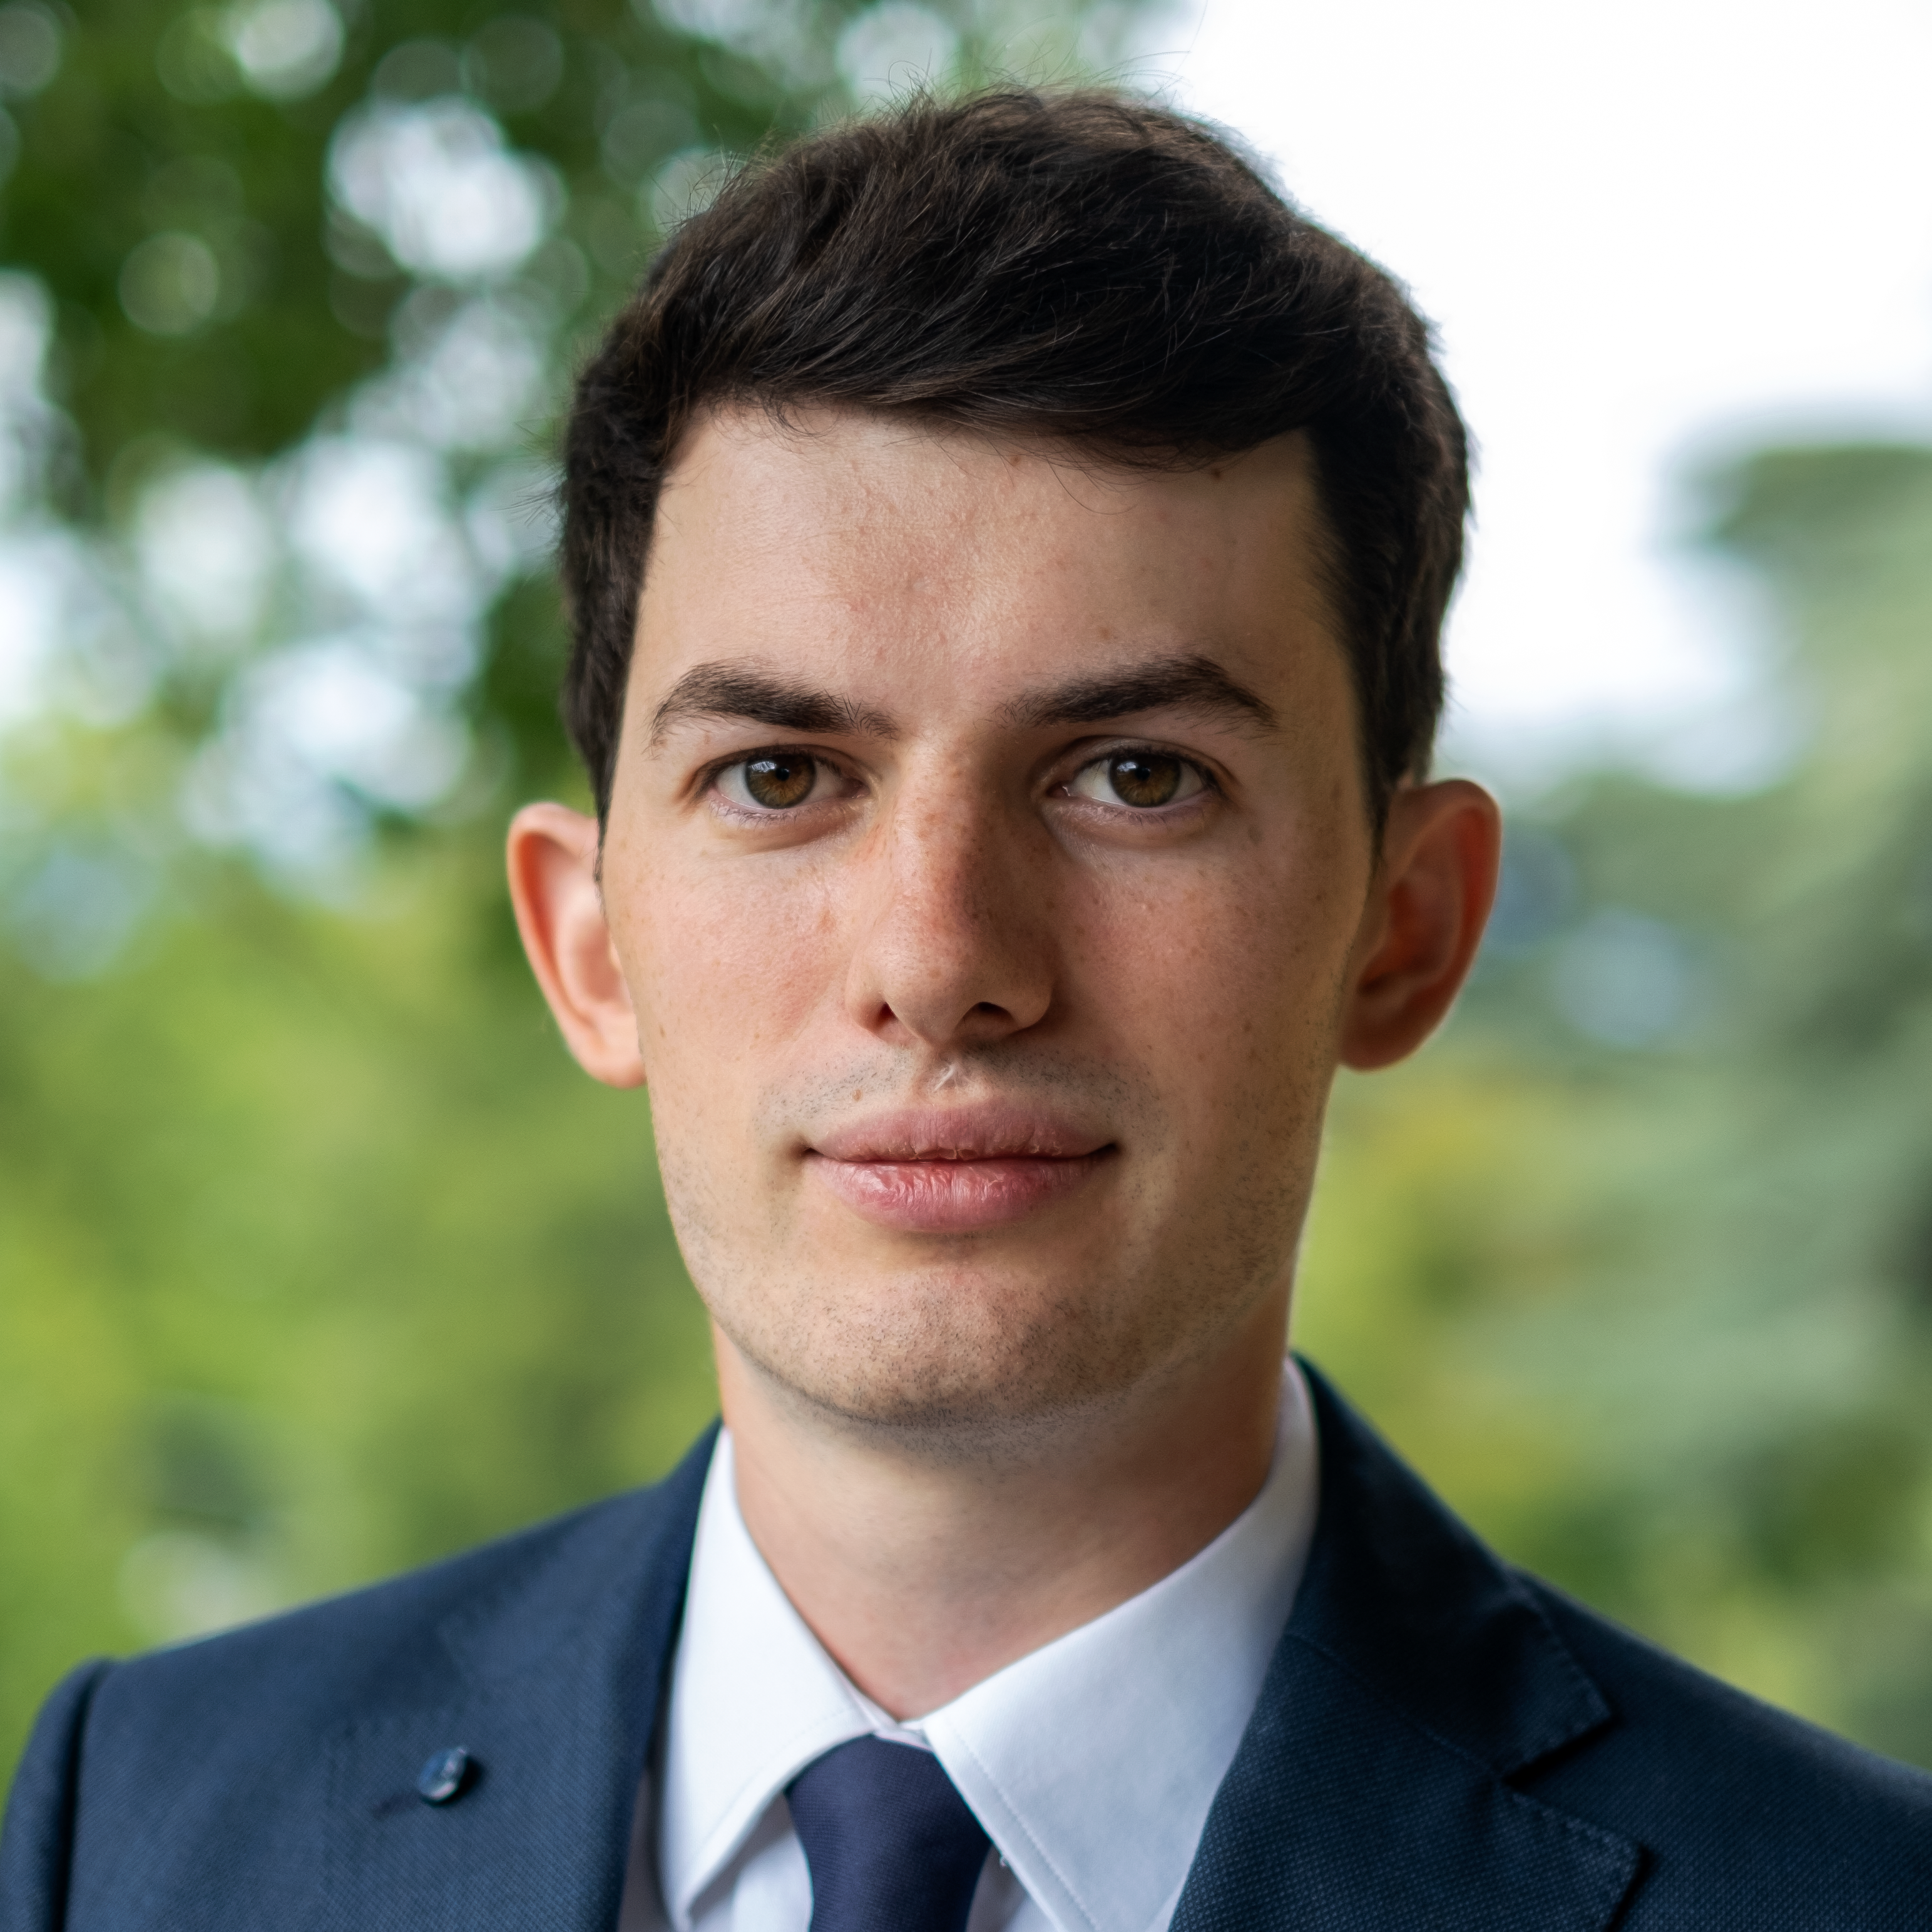
\includegraphics[width=\linewidth]{LinkedInProfilPic.png}
\end{minipage}%
\vspace{0.25cm}

\noindent\rule{\textwidth}{1pt}

% --- Section: Education ---
\begin{center}
\large\bf{EDUCATION}
\end{center}

\begin{tabularx}{1.0\textwidth} { 
   >{\raggedright\arraybackslash\hsize=1.5\hsize\linewidth=\hsize}X 
   >{\raggedleft\arraybackslash\hsize=.5\hsize\linewidth=\hsize}X }
\normalsize
\bf{Université de Genève} & Genève, CH \\
\normalfont Maîtrise universitaire\ en physique des particules & Sep 2018 -- Juin 2020  \\  
Électrodynamique quantique, Chromodynamique quantique, Théorie quantique des champs, Relativité générale, Physique des rayonnements cosmiques, Détecteurs et accélérateurs &
\end{tabularx}
\vspace{0.25cm}

\begin{tabularx}{1.0\textwidth} { 
   >{\raggedright\arraybackslash\hsize=1.5\hsize\linewidth=\hsize}X 
   >{\raggedleft\arraybackslash\hsize=.5\hsize\linewidth=\hsize}X }
\normalsize
\bf{Université de Goettingen} & Goettingen, GER \\
\normalfont Hadron collider physics school (HASCO) & Jul 2018 \\
International Student Exchange Program
\end{tabularx}
\vspace{0.25cm}

\begin{tabularx}{1.0\textwidth} { 
   >{\raggedright\arraybackslash\hsize=1.5\hsize\linewidth=\hsize}X 
   >{\raggedleft\arraybackslash\hsize=.5\hsize\linewidth=\hsize}X }
\normalsize
\bf{Université de Genève} & Genève, CH \\
\normalfont Baccalauréat universitaire\ en Physique & Sep 2015 -- Juin 2018  \\  
Mécanique newtonienne, Électrodynamique, Algèbre linéaire, Analyse complexe \& de Fourier, Astrophysiques, Mécanique statistique et Physique du solide &
\end{tabularx}
\vspace{0.25cm}

\begin{tabularx}{1.0\textwidth} { 
   >{\raggedright\arraybackslash\hsize=1.5\hsize\linewidth=\hsize}X 
   >{\raggedleft\arraybackslash\hsize=.5\hsize\linewidth=\hsize}X }
\normalsize
\bf{École Polytechnique Fédérale de Lausanne (EPFL)} & Lausanne, CH \\
\normalfont Ingénieure mécanique & Sep 2014 -- Juin 2015\\
Analyse, Algèbre linéaire, Mécanique newtonienne, Thermodynamique, 
Construction mécanique, Enjeux mondiaux, Communication, Mécanique des structures, Matériaux, Électricité
\end{tabularx}
\vspace{0.25cm}

\begin{tabularx}{1.0\textwidth} { 
   >{\raggedright\arraybackslash\hsize=1.5\hsize\linewidth=\hsize}X 
   >{\raggedleft\arraybackslash\hsize=.5\hsize\linewidth=\hsize}X }
\normalsize
\bf{École Polytechnique Fédérale de Zürich (ETH)} & Zürich, CH \\
\normalfont Ingénieure mécanique & Sep 2013 -- Juin 2014 \\
Analyse, Algèbre linéaire, Mécanique newtonienne, Matériaux et fabrication, Dessin technique \& CAD, Chimie, Éléments de machine, Informatique, Processus d'innovation \& projet
\end{tabularx}
\vspace{0.25cm}

% --- Section: Work Experience ---
\begin{center}
\noindent\rule{0.75\textwidth}{1pt}
\end{center}

\begin{center}
\large\bf{WORK EXPERIENCE}
\end{center}

\begin{tabularx}{1.0\textwidth} { 
   >{\raggedright\arraybackslash\hsize=1.5\hsize\linewidth=\hsize}X 
   >{\raggedleft\arraybackslash\hsize=.5\hsize\linewidth=\hsize}X }
\normalsize
\bf{Airline Customer Service Agent - Swissport} & Geneva, CH\\
\normalfont \begin{itemize}[leftmargin=*,noitemsep,topsep=0pt]
\item Responsible for all passenger movements between the terminal and aircraft as well as processing travel documents and assigning boarding passes
\item International airport tarmac security clearance and driving license
\item Irregular hours (evening, nights, WE, holidays)
\end{itemize} & Nov 2018 -- Present
\end{tabularx}

\begin{tabularx}{1.0\textwidth} { 
   >{\raggedright\arraybackslash\hsize=1.5\hsize\linewidth=\hsize}X 
   >{\raggedleft\arraybackslash\hsize=.5\hsize\linewidth=\hsize}X }
\normalsize
\bf{European Organization for Nuclear Research (CERN)} & Geneva, CH\\
\normalfont \begin{itemize}[leftmargin=*,noitemsep,topsep=0pt]
\item Participated in the creation of FASER, a new experiment that focuses on weakly interacting massive particles
\item Quality assurance and programming of the signal triggering system
\item Integrated my design in the workflow of a team of 30+ international scientists
\end{itemize} & Sep 2019 -- Jul 2020
\end{tabularx}

\begin{tabularx}{1.0\textwidth} { 
   >{\raggedright\arraybackslash\hsize=1.5\hsize\linewidth=\hsize}X 
   >{\raggedleft\arraybackslash\hsize=.5\hsize\linewidth=\hsize}X }
\normalsize
\bf{Physics Laboratory Assistant - University of Geneva \& ECG Jean-Piaget} & Geneva, CH\\
\normalfont \begin{itemize}[leftmargin=*,noitemsep,topsep=0pt]
\item Mentored students from high school and university to acquire and analyse data using hands-on experiments
\end{itemize} & Sep 2018 -- Aug 2020
\end{tabularx}

\begin{tabularx}{1.0\textwidth} { 
   >{\raggedright\arraybackslash\hsize=1.5\hsize\linewidth=\hsize}X 
   >{\raggedleft\arraybackslash\hsize=.5\hsize\linewidth=\hsize}X }
\normalsize
\bf{Mechanical Engineering Internship - Rolex} & Geneva, CH\\
\normalfont \begin{itemize}[leftmargin=*,noitemsep,topsep=0pt]
\item Participated in the different stages involved in the creation of high quality watches, from gold melting to ceramic milling
\end{itemize} & Jan 2014 --  Feb 2014
\end{tabularx}

\begin{tabularx}{1.0\textwidth} { 
   >{\raggedright\arraybackslash\hsize=1.5\hsize\linewidth=\hsize}X 
   >{\raggedleft\arraybackslash\hsize=.5\hsize\linewidth=\hsize}X }
\normalsize
\bf{Swiss Army - Aviation Squadron 14} & Payerne \& Sion, CH\\
\normalfont \begin{itemize}[leftmargin=*,noitemsep,topsep=0pt]
\item Aviation soldier on the F-5 Tiger and F-18 Hornet
\item Preparing the planes on-board inertial navigation system as well as refueling and hand signaling the start up procedure
\end{itemize} & Jul 2012 -- Dec 2012
\end{tabularx}

% --- Section: Additional Experience ---
\begin{center}
\noindent\rule{0.75\textwidth}{1pt}
\end{center}

\begin{center}
\large\bf{ADDITIONAL EXPERIENCE}
\end{center}

\begin{tabularx}{1.0\textwidth} { 
   >{\raggedright\arraybackslash\hsize=1.5\hsize\linewidth=\hsize}X 
   >{\raggedleft\arraybackslash\hsize=.5\hsize\linewidth=\hsize}X }
\normalsize
\bf{Expert in Radioprotection - CHUV} & Lausanne, CH\\
\normalfont \begin{itemize}[leftmargin=*,noitemsep,topsep=0pt]
\item Qualified as a radiation protection expert in the use of unsealed radioactive materials in a B/C work area
\end{itemize} & Feb -- Jul 2019
\end{tabularx}

\begin{tabularx}{1.0\textwidth} { 
   >{\raggedright\arraybackslash\hsize=1.5\hsize\linewidth=\hsize}X 
   >{\raggedleft\arraybackslash\hsize=.5\hsize\linewidth=\hsize}X }
\normalsize
\bf{Aviation Enthusiast} & Grenchen, CH\\
\normalfont \begin{itemize}[leftmargin=*,noitemsep,topsep=0pt]
\item Private Pilot License (PPL) and Aerobatics
\item Recommended by SPHAIR to become a commercial and/or a military pilot
\item Participated three times in the Swiss national aerobatics championship
\end{itemize} & 2014
\end{tabularx}


% --- Section: Skills ---
\begin{center}
\noindent\rule{0.75\textwidth}{1pt}
\end{center}

\begin{center}
\large\bf{SKILLS}
\end{center}

\begin{tabularx}{1.0\textwidth} { 
   >{\raggedright\arraybackslash\hsize=1.5\hsize\linewidth=\hsize}X 
   >{\raggedleft\arraybackslash\hsize=.5\hsize\linewidth=\hsize}X }
\normalsize
\bf{Languages} & \\
\normalfont
French - Native & \\
English - Full professional & \\
German - Intermediate 
\end{tabularx}
\vspace{0.25cm}

\begin{tabularx}{1.0\textwidth} { 
   >{\raggedright\arraybackslash\hsize=1.5\hsize\linewidth=\hsize}X 
   >{\raggedleft\arraybackslash\hsize=.5\hsize\linewidth=\hsize}X }
\normalsize
\bf{Computer Skills} & \\
\normalfont \begin{itemize}[leftmargin=*,noitemsep,topsep=0pt]
\item \textbf{Microsoft Office Suite:}  Excel, Word, PowerPoint, Outlook
\item \textbf{Programming:} C++, Python, Github
\item \textbf{Data Analysis:} Mathematica, Matlab, Root, Igor
\item \textbf{Other:} Linux, LateX, CAD, Arduino, 3D printing, Adobe Premiere, Computer building
\end{itemize} & 
\end{tabularx}

% --- Section: Publication ---
\begin{center}
\noindent\rule{0.75\textwidth}{1pt}
\end{center}

\begin{center}
\large\bf{PUBLICATION}
\end{center}

\nocite{*}

\printbibliography[title=\normalsize Master Thesis]

% --- End of CV! ---


\end{document}
